\chapter{Frequency, Phase, Domain}

\section{Frequency Decomposition}
\subsection{Review: Frequency, Hertz and Radians}
The frequency of something refers to the amount of times it occurs within a specific timeframe.
For example, a reasonable frequency for showering is one to two times per day.
However, frequency can also be used to compute the amount of time needed for a signal to reach from one peak to another peak.
The process of going from one peak in a signal wave (like a sine function) to the next peak is known as a cycle.
In science, we primarily use two units for quantifying the frequency of signals: Hertz and radians per second.

For the unit Hertz (Hz), $1 Hz$ is equivalent to $1$ cycle per second. Therefore, $1kHz$ is equivalent to $1000$ cycles per second.
On the other hand, the unit radians per second computes frequency by equating $1$ cycle to contain $2 \pi$ radians of movement.
Therefore, $1 Hz$ is equivalent to $2\pi$ radians per second

\subsection{Introduction via Signals as Musical Chords}
In music theory, musicians discuss what exactly makes a note.
Through science, we find that what defines a pitch (note), such as $C4$ (a middle $do$) or $G5$ (a high $sol$), is the pitch of such note.
Such science, psychoacoustics, claims that the way human ears can distinguish different notes within a combination of notes (for example, playing multiple keys on the piano at the same time doesn't make it impossible to identify individual notes) is because the ear helps us decompose the frequencies in a signal.
What exactly does that mean?
Let us look at the following figure, which discusses a C major chord that is made of a $C$, $E$, and $G$ note:
\begin{center}
    \begin{figure}[h]
        \centering
        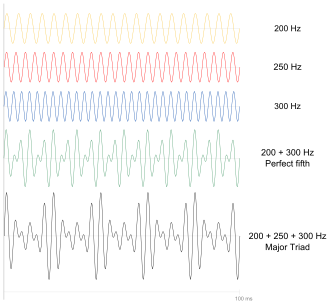
\includegraphics[width=0.7\textwidth]{figs/ln11/330px-Major_triad.svg.png}
        \caption{How individual and combined signals seem in a C major chord.}
    \end{figure}
\end{center}
In such graph, we find that the sum signal our ears perceive as a C major chord is in fact a sum of three or more signals.
Then, the ear helps us decompose this signal into three different signals; for example:
\[
    s(t) = \sin(440 \times 2\pi t) + \sin(554 \times 2\pi t) + \sin(659 \times 2\pi t)
\]
In later chapters, we will discuss how to perform this mechanically.

\subsection{Timbre}
Then, what is it that distinguishes a middle $do$ from a piano and from a violin?
The sound of different instruments when playing the same pitch is distinguished by the instruments' ``timbre'', which is a combination of frequencies uniquely pronounced by different types of instruments.
Therefore, the musical instruments are distinguishable to humans through the same frequency analysis process thatthe human ear conducts.

\section{Phase}
We have mainly visualized sound waves in sinusoidal (sine, cosine) curves.
Therefore, while considering the aplitudes, frequency of our sinusoidal waves, we may also concern its translation across time: namely, the relative starting point of a sound wave compared to other sound waves.
To express this translation, in pre-calculus syllabus, we have learned to record a signal as:
\[
    s(t) = \sin (440 \times 2 \pi t + \phi)
\]
where $\phi \in \mathbb{R}$ shows the relative start of our sound wave and is called the \textbf{phase} of our signal.

\section{Periodic and Finite Signals}
Signals that are defined on a temporal basis (or, they are time-based functions) can be categorized further.
In this section, we discuss some of these categorizations and the properties of such signals.

First, let us discuss periodic signals:
\begin{ln-define}{Periodic Signal}{}
    A periodic signal $x$ with period $p \in \mathbb{R}$ satisfies the following defining condition:
    \[
        \forall t \in \mathbb{R}, x(t) = x(t + p)
    \]
    However, such signals must also have period $2p$, as $x(t + 2p) = x((t+p) + p) = x(t+p) = x(t)$.
    Therefore, we define the period of a periodic signal to be the smallest positive value $p$ such that the defining condition of periodic signal is satisfied.
\end{ln-define}

A periodic signal, therefore, ought to be defined over an infinite interval: it is defined at any possible real time.
On the other hand, some signals' domain may be a subset of real numbers.
In such case, we say this signal is a \textbf{finite signal}.
And, essentially, any periodic signal is the infinite repetition of some finite signal.
